\documentclass[14pt]{extbook}
\usepackage{multicol, enumerate, enumitem, hyperref, color, soul, setspace, parskip, fancyhdr} %General Packages
\usepackage{amssymb, amsthm, amsmath, bbm, latexsym, units, mathtools} %Math Packages
\everymath{\displaystyle} %All math in Display Style
% Packages with additional options
\usepackage[headsep=0.5cm,headheight=12pt, left=1 in,right= 1 in,top= 1 in,bottom= 1 in]{geometry}
\usepackage[usenames,dvipsnames]{xcolor}
\usepackage{dashrule}  % Package to use the command below to create lines between items
\newcommand{\litem}[1]{\item#1\hspace*{-1cm}\rule{\textwidth}{0.4pt}}
\pagestyle{fancy}
\lhead{Progress Quiz 8}
\chead{}
\rhead{Version C}
\lfoot{4553-3922}
\cfoot{}
\rfoot{Fall 2020}
\begin{document}

\begin{enumerate}
\litem{
Determine the domain of the function below.\[ f(x) = \frac{5}{25x^{2} +55 x + 30} \]\begin{enumerate}[label=\Alph*.]
\item \( \text{All Real numbers except } x = a, \text{ where } a \in [-1.43, -1.16] \)
\item \( \text{All Real numbers except } x = a \text{ and } x = b, \text{ where } a \in [-30.2, -29.61] \text{ and } b \in [-25.05, -24.65] \)
\item \( \text{All Real numbers except } x = a, \text{ where } a \in [-30.2, -29.61] \)
\item \( \text{All Real numbers.} \)
\item \( \text{All Real numbers except } x = a \text{ and } x = b, \text{ where } a \in [-1.43, -1.16] \text{ and } b \in [-1.04, -0.29] \)

\end{enumerate} }
\litem{
Solve the rational equation below. Then, choose the interval(s) that the solution(s) belongs to.\[ \frac{-5}{9x -2} + 9 = \frac{5}{-63x + 14} \]\begin{enumerate}[label=\Alph*.]
\item \( \text{All solutions lead to invalid or complex values in the equation.} \)
\item \( x \in [0.28,1.28] \)
\item \( x_1 \in [0, 0.7] \text{ and } x_2 \in [0.28,0.41] \)
\item \( x \in [-0.7,0] \)
\item \( x_1 \in [-0.7, 0] \text{ and } x_2 \in [0.26,0.31] \)

\end{enumerate} }
\litem{
Solve the rational equation below. Then, choose the interval(s) that the solution(s) belongs to.\[ \frac{-4x}{-5x + 5} + \frac{-6x^{2}}{25x^{2} +5 x -30} = \frac{6}{-5x -6} \]\begin{enumerate}[label=\Alph*.]
\item \( x \in [-2.6,-0.3] \)
\item \( x \in [-7.5,-2.7] \)
\item \( \text{All solutions lead to invalid or complex values in the equation.} \)
\item \( x_1 \in [0.1, 1] \text{ and } x_2 \in [-6.35,-0.35] \)
\item \( x_1 \in [0.1, 1] \text{ and } x_2 \in [-1,4] \)

\end{enumerate} }
\litem{
Choose the graph of the equation below.\[ f(x) = \frac{1}{(x - 1)^2} + 2 \]\begin{enumerate}[label=\Alph*.]
\begin{multicols}{2}\item 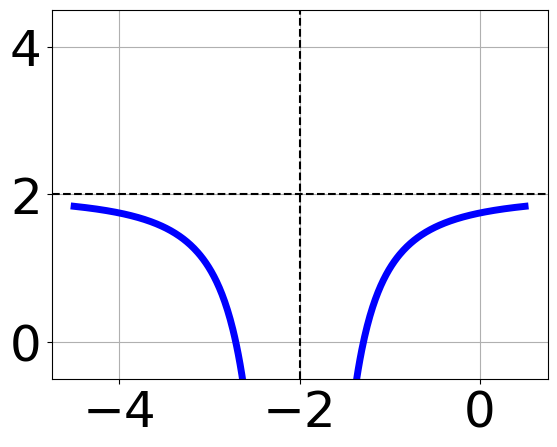
\includegraphics[width = 0.3\textwidth]{../Figures/rationalEquationToGraphCopyAC.png}\item 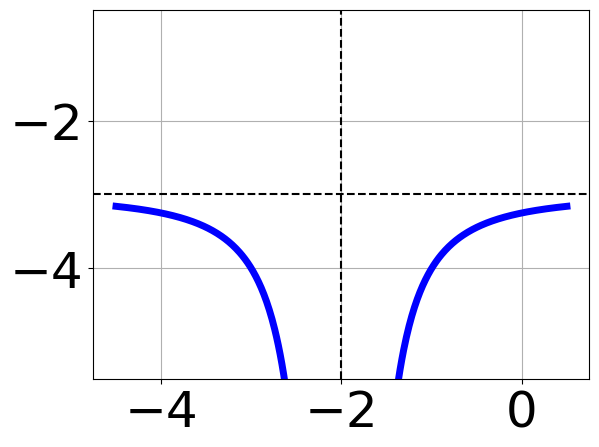
\includegraphics[width = 0.3\textwidth]{../Figures/rationalEquationToGraphCopyBC.png}\item 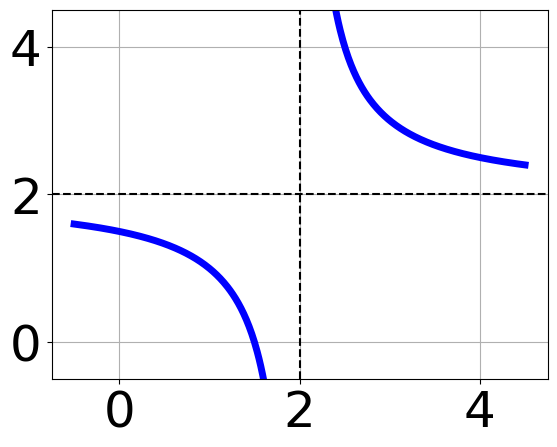
\includegraphics[width = 0.3\textwidth]{../Figures/rationalEquationToGraphCopyCC.png}\item 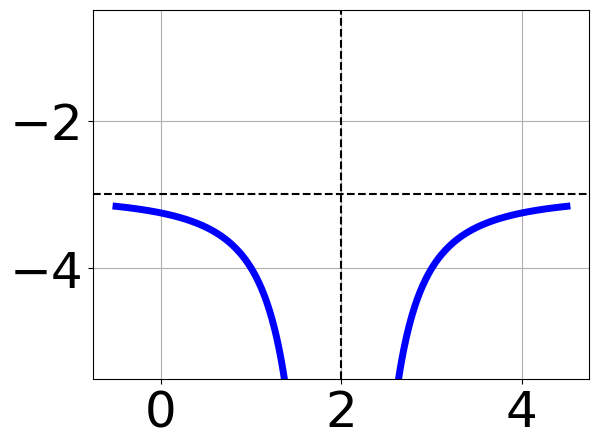
\includegraphics[width = 0.3\textwidth]{../Figures/rationalEquationToGraphCopyDC.png}\end{multicols}\item None of the above.
\end{enumerate} }
\litem{
Choose the equation of the function graphed below.
\begin{center}
    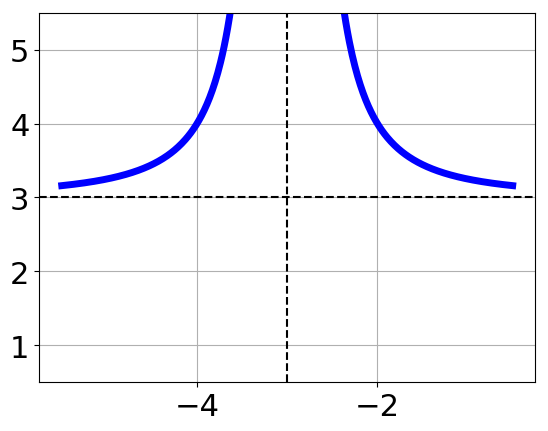
\includegraphics[width=0.5\textwidth]{../Figures/rationalGraphToEquationC.png}
\end{center}
\begin{enumerate}[label=\Alph*.]
\item \( f(x) = \frac{-1}{x - 3} + 2 \)
\item \( f(x) = \frac{-1}{(x - 3)^2} + 2 \)
\item \( f(x) = \frac{1}{(x + 3)^2} + 2 \)
\item \( f(x) = \frac{1}{x + 3} + 2 \)
\item \( \text{None of the above} \)

\end{enumerate} }
\litem{
Choose the graph of the equation below.\[ f(x) = \frac{-1}{(x + 2)^2} + 2 \]\begin{enumerate}[label=\Alph*.]
\begin{multicols}{2}\item 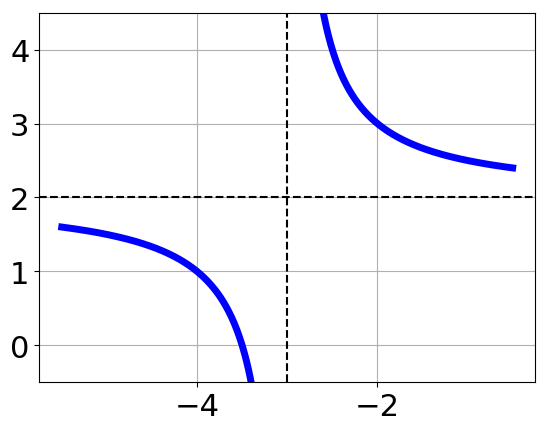
\includegraphics[width = 0.3\textwidth]{../Figures/rationalEquationToGraphAC.png}\item 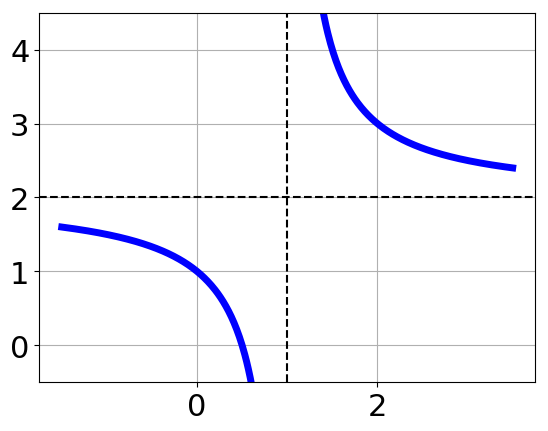
\includegraphics[width = 0.3\textwidth]{../Figures/rationalEquationToGraphBC.png}\item 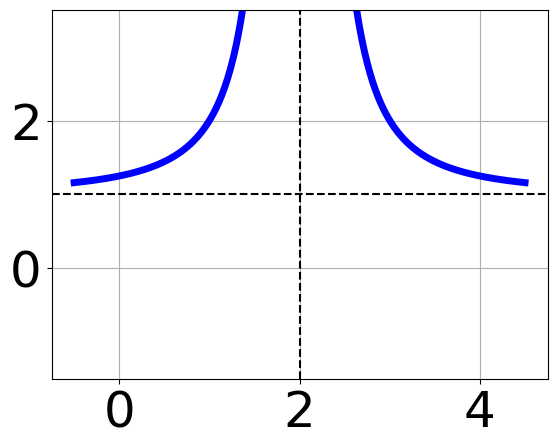
\includegraphics[width = 0.3\textwidth]{../Figures/rationalEquationToGraphCC.png}\item 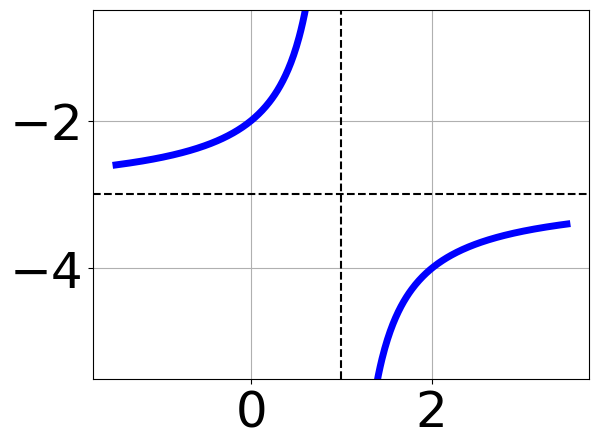
\includegraphics[width = 0.3\textwidth]{../Figures/rationalEquationToGraphDC.png}\end{multicols}\item None of the above.
\end{enumerate} }
\litem{
Solve the rational equation below. Then, choose the interval(s) that the solution(s) belongs to.\[ \frac{6x}{-6x -6} + \frac{-4x^{2}}{30x^{2} +48 x + 18} = \frac{4}{-5x -3} \]\begin{enumerate}[label=\Alph*.]
\item \( x_1 \in [-2.26, -0.66] \text{ and } x_2 \in [-7,0] \)
\item \( x \in [0.19,2.22] \)
\item \( \text{All solutions lead to invalid or complex values in the equation.} \)
\item \( x_1 \in [-2.26, -0.66] \text{ and } x_2 \in [0.93,5.93] \)
\item \( x \in [-0.63,-0.06] \)

\end{enumerate} }
\litem{
Choose the equation of the function graphed below.
\begin{center}
    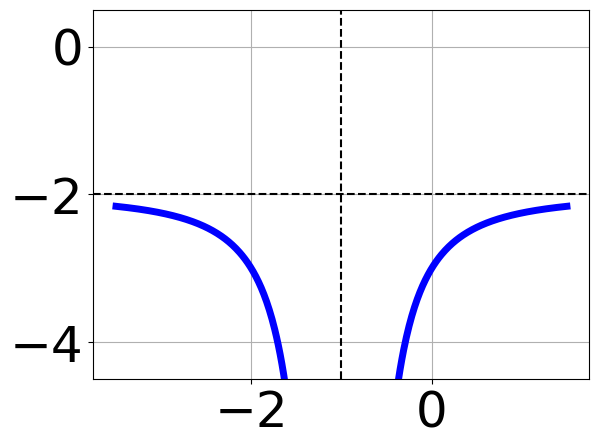
\includegraphics[width=0.5\textwidth]{../Figures/rationalGraphToEquationCopyC.png}
\end{center}
\begin{enumerate}[label=\Alph*.]
\item \( f(x) = \frac{-1}{(x + 1)^2} + 2 \)
\item \( f(x) = \frac{-1}{x + 1} + 2 \)
\item \( f(x) = \frac{1}{x - 1} + 2 \)
\item \( f(x) = \frac{1}{(x - 1)^2} + 2 \)
\item \( \text{None of the above} \)

\end{enumerate} }
\litem{
Determine the domain of the function below.\[ f(x) = \frac{4}{30x^{2} -48 x + 18} \]\begin{enumerate}[label=\Alph*.]
\item \( \text{All Real numbers except } x = a \text{ and } x = b, \text{ where } a \in [14.83, 15.94] \text{ and } b \in [35.83, 36.19] \)
\item \( \text{All Real numbers except } x = a, \text{ where } a \in [14.83, 15.94] \)
\item \( \text{All Real numbers.} \)
\item \( \text{All Real numbers except } x = a, \text{ where } a \in [0.43, 0.72] \)
\item \( \text{All Real numbers except } x = a \text{ and } x = b, \text{ where } a \in [0.43, 0.72] \text{ and } b \in [0.7, 1.44] \)

\end{enumerate} }
\litem{
Solve the rational equation below. Then, choose the interval(s) that the solution(s) belongs to.\[ \frac{3}{5x -9} + 5 = \frac{4}{-40x + 72} \]\begin{enumerate}[label=\Alph*.]
\item \( x_1 \in [-3.94, -0.94] \text{ and } x_2 \in [1.65,1.71] \)
\item \( x \in [-3.94,-0.94] \)
\item \( \text{All solutions lead to invalid or complex values in the equation.} \)
\item \( x_1 \in [1.66, 2.66] \text{ and } x_2 \in [1.79,2.05] \)
\item \( x \in [1.66,2.66] \)

\end{enumerate} }
\end{enumerate}

\end{document}